
\documentclass[
	% -- opções da classe memoir --
	12pt,				% tamanho da fonte
	openright,			% capítulos começam em pág ímpar (insere página vazia caso preciso)
	oneside,			% para impressão em apenas anverso. Oposto a twoside
	%twoside,			% para impressão em verso e anverso. Oposto a oneside
	a4paper,			% tamanho do papel. 
	% -- opções da classe abntex2 --
	%chapter=TITLE,		% títulos de capítulos convertidos em letras maiúsculas
	%section=TITLE,		% títulos de seções convertidos em letras maiúsculas
	%subsection=TITLE,	% títulos de subseções convertidos em letras maiúsculas
	%subsubsection=TITLE,% títulos de subsubseções convertidos em letras maiúsculas
	% -- opções do pacote babel --
	english,			% idioma adicional para hifenização
	brazil				% o último idioma é o principal do documento
]{abntex2}

% Evita linhas orfãs e viúvas
\widowpenalty=10000
\clubpenalty=10000

\usepackage[subentrycounter,seeautonumberlist,nonumberlist=true]{glossaries}
%\usepackage{lmodern}			% Usa a fonte Latin Modern
\usepackage{helvet}
\renewcommand{\familydefault}{\sfdefault}
\usepackage[T1]{fontenc}		% Selecao de codigos de fonte.
\usepackage[utf8]{inputenc}		% Codificacao do documento (conversão automática dos acentos)
\usepackage{lastpage}			% Usado pela Ficha catalográfica
\usepackage{indentfirst}		% Indenta o primeiro parágrafo de cada seção.
\usepackage{color, colortbl}
% Controle das cores
\definecolor{LightCyan}{rgb}{0.88,1,1} %Cor ciano
\definecolor{Blue}{rgb}{0,0,1} %Cor ciano
\usepackage{graphicx}			% Inclusão de gráficos
\usepackage{microtype} 			% para melhorias de justificação
\usepackage{lipsum}				% para geração de dummy text
\usepackage[alf,abnt-etal-list=0,abnt-etal-cite=3,abnt-etal-text=emph]{abntex2cite}					% Citações padrão ABNT
\usepackage{tikz}
\usepackage{svg}
\usetikzlibrary{shapes,arrows,chains}
\usepackage[]{mcode}
\usepackage{multirow}
\usepackage{booktabs}
\usepackage{array}
\usepackage{longtable}
\usepackage{rotating}
\usepackage[small]{caption}
\usepackage{pbox}
\usepackage{pdfpages}
\usepackage{float}
\usepackage{amsmath, esint}
\usepackage{multicol}
\usepackage{adjustbox}
\usepackage{todonotes}
\usepackage{gensymb}
\usepackage[thinc]{esdiff}

\usepackage{soul}
\usepackage[brazil]{babel}
\usepackage{blindtext}[]

\usepackage{caption}
\usepackage{subcaption}

\newcommand{\?}{\ensuremath{\texttt{\textbf{CITATION~NEEDED}}}}
\newcommand{\oautor}{Fonte: o Autor, 2021.}



%\newcommand{\hlg}[1]{{\colorbox{green}{#1}}}
%\newcommand{\hls}[1]{{\colorbox{yellow}{#1}}}
%\newcommand{\hli}[1]{{\colorbox{lime}{#1}}}
\newcommand{\hlg}[1]{{\colorbox{white}{#1}}}
\newcommand{\hls}[1]{{\colorbox{white}{#1}}}
\newcommand{\hli}[1]{{\colorbox{white}{#1}}}


\counterwithout{equation}{chapter}

\graphicspath{
	{../Mathematica}
	{../Mathematica/Images}
	{../Classifier/Graphs}
}

%\usepackage[brazil]{babel}		% idiomas
\addto\captionsbrazil{
	%% ajusta nomes padroes do babel
	\renewcommand{\bibname}{Refer\^encias Bibliogr\'aficas}
	\renewcommand{\indexname}{\'Indice Remissivo}
	\renewcommand{\listfigurename}{Lista de Figuras}
	\renewcommand{\listtablename}{Lista de Tabelas}
	\renewcommand{\listadesiglasname}{Lista de Abreviaturas e Siglas}
	%% ajusta nomes usados com a macro \autoref
	\renewcommand{\pageautorefname}{p\'agina}
	\renewcommand{\sectionautorefname}{se{\c c}\~ao}
	\renewcommand{\subsectionautorefname}{subse{\c c}\~ao}
	\renewcommand{\paragraphautorefname}{par\'agrafo}
	\renewcommand{\subsubsectionautorefname}{subse{\c c}\~ao}
}

\newenvironment{listofabbrv}[1]{
        \chapter*{Lista de abreviaturas}
        \begin{list}{\textbf{??}}{
                \settowidth{\labelwidth}{#1}
                \setlength{\labelsep}{1em}
                \setlength{\itemindent}{0mm}
                \setlength{\leftmargin}{\labelwidth}
                \addtolength{\leftmargin}{\labelsep}
                \setlength{\rightmargin}{0mm}
                \setlength{\itemsep}{.1\baselineskip}
                \renewcommand{\makelabel}[1]{\makebox[\labelwidth][l]{##1}}
        }
}{
        \end{list}
}

\definecolor{blue}{RGB}{0,114,189}
\definecolor{orange}{RGB}{217,83,25}
\definecolor{yellow}{RGB}{237,177,32}
\definecolor{purple}{RGB}{126,47,142}
\definecolor{green}{RGB}{119,172,48}
\definecolor{lightBlue}{RGB}{77,190,238}
\definecolor{red}{RGB}{162,20,47}
\definecolor{black}{RGB}{0,0,0}

% informações do PDF
\makeatletter
\hypersetup{
     	%pagebackref=true,
		pdftitle={\@title}, 
		pdfauthor={\@author},
    	pdfsubject={\imprimirpreambulo},
	    pdfcreator={LaTeX},
		pdfkeywords={abnt}{latex}{abntex}{abntex2}{trabalho acadêmico}, 
		colorlinks=true,	% false: boxed links; true: colored links
    	linkcolor=black,	% color of internal links
    	citecolor=black,	% color of links to bibliography
    	filecolor=black,	% color of file links
		urlcolor=black,
		bookmarksdepth=4
}
\makeatother

% --- 
% Espaçamentos entre linhas e parágrafos 
% --- 
% O tamanho do parágrafo é dado por:
\setlength{\parindent}{1.3cm}
% Controle do espaçamento entre um parágrafo e outro:
\setlength{\parskip}{0.2cm}  % tente também \onelineskip

\lstset{literate=
  {á}{{\'a}}1 {é}{{\'e}}1 {í}{{\'i}}1 {ó}{{\'o}}1 {ú}{{\'u}}1
  {ã}{{\~a}}1 {õ}{{\~o}}1
  {Á}{{\'A}}1 {É}{{\'E}}1 {Í}{{\'I}}1 {Ó}{{\'O}}1 {Ú}{{\'U}}1
  {à}{{\`a}}1 {è}{{\`e}}1 {ì}{{\`i}}1 {ò}{{\`o}}1 {ù}{{\`u}}1
  {À}{{\`A}}1 {È}{{\'E}}1 {Ì}{{\`I}}1 {Ò}{{\`O}}1 {Ù}{{\`U}}1
  {ä}{{\"a}}1 {ë}{{\"e}}1 {ï}{{\"i}}1 {ö}{{\"o}}1 {ü}{{\"u}}1
  {Ä}{{\"A}}1 {Ë}{{\"E}}1 {Ï}{{\"I}}1 {Ö}{{\"O}}1 {Ü}{{\"U}}1
  {â}{{\^a}}1 {ê}{{\^e}}1 {î}{{\^i}}1 {ô}{{\^o}}1 {û}{{\^u}}1
  {Â}{{\^A}}1 {Ê}{{\^E}}1 {Î}{{\^I}}1 {Ô}{{\^O}}1 {Û}{{\^U}}1
  {œ}{{\oe}}1 {Œ}{{\OE}}1 {æ}{{\ae}}1 {Æ}{{\AE}}1 {ß}{{\ss}}1
  {ű}{{\H{u}}}1 {Ű}{{\H{U}}}1 {ő}{{\H{o}}}1 {Ő}{{\H{O}}}1
  {ç}{{\c c}}1 {Ç}{{\c C}}1 {ø}{{\o}}1 {å}{{\r a}}1 {Å}{{\r A}}1
  {€}{{\euro}}1 {£}{{\pounds}}1,
  language=Python, extendedchars=true, breaklines=true
}

% colorir códigos
\usepackage{listings}
\renewcommand{\lstlistingname}{Quadro}
\definecolor{codebackground}{rgb}{0.95,0.95,0.92}
\definecolor{numberscolor}{rgb}{0.21, 0.27, 0.31}
\definecolor{pythoncomment}{rgb}{0,0.6,0}
\definecolor{pythonstring}{rgb}{0.58,0,0.82}
\definecolor{csharpcomment}{rgb}{0, 0.5, 0}
\definecolor{csharpdocumentation}{rgb}{0.3, 0.3, 0.3}
\definecolor{csharptype}{rgb}{0.17, 0.57, 0.69}
\definecolor{csharpkeyword}{rgb}{0, 0, 1}
\definecolor{csharpstring}{rgb}{0.64, 0.08, 0.08}
\definecolor{innosetupkeyword}{rgb}{0, 0.35, 0.67}
\definecolor{innosetupsections}{rgb}{0, 0, 0.5}
\definecolor{xamlkeyword}{rgb}{0.5,0,0}
\definecolor{xamlcomment}{rgb}{0,0.5,0}
\lstloadlanguages{Python,csh,C,C++, XML, Verilog}

\lstdefinestyle{VerilogStyle}{
    language=Verilog,
    backgroundcolor=\color{codebackground},
    commentstyle=\color{csharpcomment},
    keywordstyle=\color{csharpkeyword},
    numberstyle=\scriptsize\color{numberscolor},
    identifierstyle=\color{black},
    stringstyle=\color{csharpstring}\ttfamily,
    basicstyle=\linespread{0.9}\ttfamily\small,
    moredelim=[l][\color{csharpdocumentation}]{///}, % Cor customizada para apresentar documentação de maneira independente
    breakatwhitespace=false,
    breaklines=true,
    captionpos=b,
    keepspaces=true,
    numbers=left,
    numbersep=5pt,
    showspaces=false,
    showstringspaces=false,
    showtabs=false,
    tabsize=2,
    extendedchars=true,
    xleftmargin=17pt,
    framexleftmargin=17pt,
    framexrightmargin=5pt,
    framexbottommargin=4pt,
    morecomment=[l]{//\ }, % Comentários de 1 linha devem ter espaço após as duas barras, para não misturar com documentação que usa 3 barras
    morecomment=[s]{/*}{*/}, % Comentário multilinha
    showstringspaces=false,
}

% Para revisão

%% Use "final" option to remove all tracking markups
%\usepackage[final]{changes}
%\definechangesauthor[name={Valner}, color=red]{vb}
%\usepackage[final]{changes}
%\deleted[id=A]{}
%\added[id=A]{}

\titulo{
Ensaio sobre os Efeitos de Envelhecimento Acelerado Decorrentes de BTI em Circuitos Digitais
}
\autor
{
	UNIVERSIDADE FEDERAL DO RIO GRANDE DO SUL\\
	ESCOLA DE ENGENHARIA\\
	DEPARTAMENTO DE ENGENHARIA ELÉTRICA\\
	\vspace*{4\baselineskip} 
    Murilo Eduardo Reinicke
}
\local{Porto Alegre}
\data{2024}
\orientador{Prof. Dr. Tiago Roberto Balen}
\instituicao{UFRGS}
\preambulo{Projeto de Diplomação, apresentado ao Departamento de Engenharia Elétrica da Escola de Engenharia da Universidade Federal do Rio Grande do Sul, como requisito para a obtenção do grau de Engenheiro Eletricista}

% ---
% INDICE
% ---
\makeindex
% ---
% GLOSSARIO
% ---
\makeglossaries

% Exemplo de configurações do glossairo
\renewcommand*{\glsseeformat}[3][\seename]{\textit{#1}  
\glsseelist{#2}}

\begin{document}

\selectlanguage{brazil}
%\selectlanguage{english}
\frenchspacing 

\imprimircapa
\imprimirfolhaderosto*

%\begin{fichacatalografica}
%	\includepdf{FC.pdf}
%\end{fichacatalografica}

%%======================
%% FOLHA DE APROVAÇÃO
%%=====================

%\begin{folhadeaprovacao}
%	\begin{center}
%		{\ABNTEXchapterfont\large{Eduarda de Castro Guterres}}
		
%		\vspace*{\fill}
%		\begin{center}
%			\ABNTEXchapterfont\bfseries\Large\imprimirtitulo
%		\end{center}
		
%		\vspace*{\fill}
%		\hspace{.45\textwidth}
%		\begin{minipage}{.5\textwidth}
%			\imprimirpreambulo
%		\end{minipage}%
%	\end{center}
	

	%\assinatura{\textbf{Prof. Dr. Ály Ferreira Flores Filho} \\ Chefe do Departamento de Engenharia Elétrica (DELET) - UFRGS}
%	
%   
%	
 %  \begin{center}
%	BANCA EXAMINADORA
	
  %\assinatura{\textbf{Prof. Dr. Giovani Bulla} \\ UFRGS}
%	\assinatura{\textbf{Prof. Dr. Alexandre Balbinot} \\ UFRGS}
	
%	\assinatura{\textbf{Profª. Dra. Adriane Parraga} \\ UERGS}
	
%	\assinatura{\textbf{\imprimirorientador} \\ Orientador - UFRGS} 
	
 %  \end{center}
  
 %\begin{center}
%	Aprovado em 21 de Maio de 2021.
%	\end{center}
%\end{folhadeaprovacao}
%================
% AGRADECIMENTOS
%=================

%\begin{agradecimentos}
%	\blindtext
    

%\end{agradecimentos}

%==========
% Resumo / Abstract
%===========

% resumo em português
\begin{resumo}[Resumo]
% O presente trabalho tem como objetivo estudar o comportamento de FPGAs afetados por envelhecimento acelerado, mais especificamente através do fenômeno de BTI, ou Bias-Temperature Instability que ocorre em decorrência da operação do dispositivo em ambientes de alta temperatura e sobre tensão de alimentação. Consequentemente uma variação na tensão de treashold ocorre nos transistores que compõe o componente. Serão ensaiados dois FPGAs: o Cyclone II da Altera e o Kintex 7 da Xilinx, ambos de tecnologia CMOS, com nó tecnológico de, respectivamente 90nm e 28nm. Os ensaios consistirão em sintetizar circuitos osciladores em anel nos dispositivos e submete-los a alta temperatura em uma câmara térmica. Após uma quantidade a ser determinada de ciclos estresse e relaxamento a frequência de oscilação será medida e será verificado se houve uma degradação na performance dele. Também será verificado se houve uma diferença relevante entre os dois dispositivos.

    \vspace{\onelineskip}
	\noindent
        
	\textbf{Palavras-chave}: Envelhecimento Acelerado, Bias-Temperature Instability, Osciladores em Anel.

\end{resumo}

\setlength{\absparsep}{18pt} 

%=======================
% SUMÁRIOS
%========================
% inserir o sumario
\pdfbookmark[0]{\contentsname}{toc}
\tableofcontents*
\cleardoublepage

% inserir lista de ilustrações
\pdfbookmark[0]{\listfigurename}{lof}
\listoffigures*
\cleardoublepage

% inserir lista de tabelas
\pdfbookmark[0]{\listtablename}{lot}
\listoftables*
\cleardoublepage

\begin{comment} 


%insere lista de abreviaturas
\pdfbookmark[0]{\listadesiglasname}{toc}
\input{chapters/06_abbreviations.tex}
\cleardoublepage



\textual
\end{comment} 
%=====================
%CHAPTERS
%====================

% %====================
% INTRODUÇÃO
	\chapter{Introdução}
%=================

A cada dia que passa mais e mais sistemas embarcados estão fazendo parte de nossas vidas, desempenhando papéis que vão de aplicações rotineiras como computadores e aparelhos celulares a aplicações críticas como tecnologia aeroespacial e médica, os sistemas estão cada vez mais complexos.

Em aplicações críticas, a confiabilidade é essencial para garantir a segurança e a saúde das pessoas. Por exemplo, em equipamentos médicos, como monitores de sinais vitais ou respiradores mecânicos, falhas podem levar a resultados graves, e até mesmo fatais. Da mesma forma, em sistemas aeronáuticos, falhas podem resultar em acidentes com consequências desastrosas.

No entanto, esses sistemas embarcados muitas vezes atuam em ambientes hostis e que pode decorrer um envelhecimento acelerado e em degradação da funcionalidade ao longo do tempo.

Um dos principais fenômenos que podem ocorrer é o BTI (bias-temperature instability) que consequentemente aumenta a variação de tensão de threshold (∆Vth) dos transistores p e transistores n que constituem o dispositivo, o que acarreta em uma menor velocidade de transição de aberto para fechado (ou de fechado para aberto) podendo depreciar a performance do sistema como um todo.

Sabendo disso, é de grande importância entender a mudança de comportamento desses sistemas para ser possível realizar projetos com maior previsibilidade e robustez, consequentemente tornando viáveis produtos mais duráveis e seguros.

Com isso, o trabalho tem como objetivo estudar os efeitos do envelhecimento em sistemas em chip de, pelo menos, dois diferentes nós tecnológicos de CMOS, XXnm e YYnm.

Para isso foram definidos os seguintes objetivos específicos:
\begin{itemize}
    \item Desenvolvimento de oscilador em anel sintetizado utilizando linguagem de descrição de hardware;
    \item Exposição dos componentes a envelhecimento acelerado;
    \item Verificação na degradação da performance;
\end{itemize}

\chapter{Fundamentação Teórica e Revisão Bibliográfica}

\section{FPGAs}

FPGA, ou \textit{Field Programmable Gate Arrays}, são dispositivos eletrônicos que são baseados em matrizes de blocos lógicos configuráveis que são conectados via interconexões programáveis \cite{AmdFpga}. Eles podem ser programados e reprogramados para as funcionalidades desejadas.

Sua utilização é necessária em aplicações onde uma implementação em \textit{software} utilizando um microcontrolador não é capaz de cumprir os requisitos de frequência de operação \cite{Sulaiman}.

O que cada bloco lógico possui internamente depende da fabricante e modelo do dispositivo, mas de forma geral possuem pelo menos \textit{Look-Up Tables} (LUTs), que são implementações em hardware de tabelas verdade e elementos de memória, como Flip-Flops \cite{Sato}.

A Figura \ref{fig:FPGAStructure} ilustra a estrutura básica de um FPGA mostrando os blocos lógicos configuráveis, as conexões programáveis.

\begin{figure}[H]
    \centering
    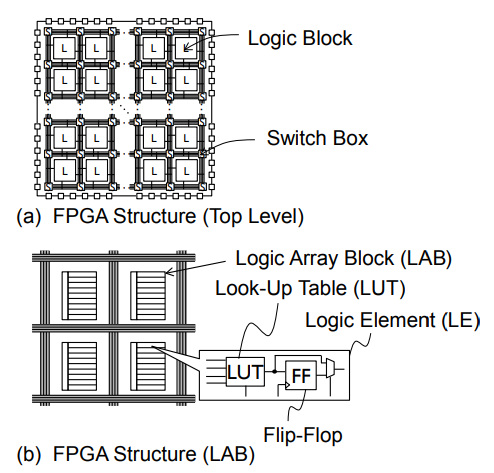
\includegraphics[scale=0.5]{figures/ReferencialTeorico/FPGAStructure.png}
    \caption{Estrutura de um FPGA. Fonte: \cite{Sato}}
    \label{fig:FPGAStructure}
\end{figure}

Os FPGAs são, de forma geral, programados utilizando linguagens de descrição de \textit{hardware} (HDL), sendo VHDL e Verilog as mais utilizadas \cite{Ain}. Essas linguagens, diferentemente de linguagens de programação convencionais onde se escreve uma série de comandos que serão executados de maneira sequencial, descrevem um circuito elétrico que será sintetizado no dispositivo.

A linguagem VHDL é pode ser utilizada para modelar sistemas digitais em diversos níveis de abstração indo do nível de algoritmo ao nível de portas lógicas. A complexidade pode variar do mais simples ao mais complexo \cite{Wunnava}. A Figura \ref{fig:Vhdl} mostra que a linguagem VHDL também pode ser definida como uma combinação de linguagens quando consideramos o nível de abstração.

\begin{figure}[H]
    \centering
    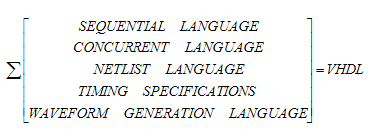
\includegraphics[scale=0.8]{figures/ReferencialTeorico/Vhdl.png}
    \caption{Integração de linguagens que constituem o VHDL. Fonte: \cite{Wunnava}}
    \label{fig:Vhdl}
\end{figure}

% VHDL is a hardware description language employed to model a digital system or digital hardware device at many levels of abstraction, ranging from the algorithmic level to the gate level (Bhasker, 1999a). The complexity of the digital system being modeled could vary from that of a simple gate to a complete digital electronic  system,  or  anything  in  between.  The  digital  system  can  also  be  described  hierarchically.  The VHDL language can also be described as a combination of languages as shown in Figure 1.

A linguagem Verilog permite descrever sistemas digitais desde o nível de portas lógicas ao nível de algoritmo. Também descreve um design do ponto de vista comportamental, de fluxo de dados, estrutural e de atrasos \cite{Bhasker}. Além disso, define sintaxe, semântica e estrutura para realizar simulações, facilitando os testes, em nível de simulação, antes da prototipação e possui simbologia e estrutura parecida com a linguagem C, tornando-se mais familiar para quem for utilizá-la \cite{Wunnava}.

\section{Oscilador em Anel}
O oscilador em anel é uma topologia de circuito muito utilizada para a caracterização de parâmetros de circuito de diversos tipos. Um dos principais motivos para isso é a capacidade de representar uma aplicação operando em alta velocidade. Segundo \cite{Bhushan} medidas feitas sob estas condições são mais próximas das aplicações reais da tecnologia do que parametrização dc convencionais, o que é verdade principalmente para dispositivos CMOS de alta performance.

Eles também são utilizados como sensores de alta precisão que aumentam a confiabilidade de um chip, podendo ser usado para monitorar diversos parâmetros como variações de processo, temperatura e efeitos de envelhecimento \cite{Sato}. Podem ser facilmente implementados e possuem um consumo de energia pequeno.

O circuito do oscilador em anel consiste em portas lógicas inversoras ligadas em sequência com uma realimentação entre a saída da última e a entrada da primeiro. É necessário que haja um número ímpar de inversores, para assim haver uma inversão periódica da entrada e da saída. O atraso de propagação de cada inversor e a realimentação gera uma onda quadrada na saída.

O período da oscilação é duas vezes o somatório do atraso de cada inversor. A Equação \ref{eq:TotalDelay} mostra frequência de oscilação, considerando que todos os inversores têm o mesmo atraso, onde N representa o número de inversores e Ta representa o tempo de atraso de um inversor.

\begin{equation}
    F = \frac{1}{2.N.Ta}
    \label{eq:TotalDelay}
\end{equation}
         
A Figura \ref{fig:RingOsc} mostra o diagrama do oscilador em anel. O circuito em questão também possui um sinal de \textit{enable}, que, além de servir para controlar o funcionamento do oscilador, também evita que o circuito entre em um estado de metaestabilidade e não oscile.

\begin{figure}[H]
    \centering
    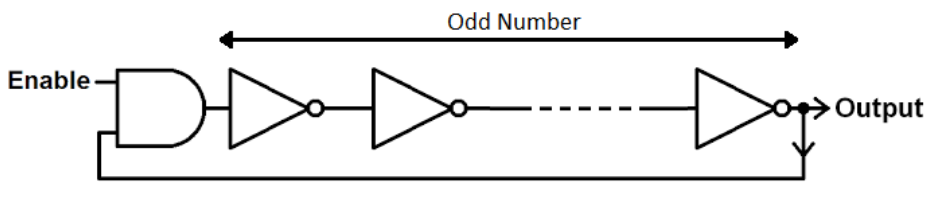
\includegraphics[width=\linewidth]{figures/ReferencialTeorico/RingOscModified.png}
    \caption{Oscilador em Anel. Fonte: \cite{Sparkfun}, modificado pelo autor}
    \label{fig:RingOsc}
\end{figure}

Uma quantidade na casa das centenas de inversores no circuito reduzirá as variações aleatórias intrínsecas de cada MOSFET que poderiam aparecer caso fossem medidos individualmente, permitindo uma caracterização mais confiável e robusta.

O trabalho de \cite{Bhushan} descreve estratégias de design para estruturas de osciladores em anel e também apresenta o uso dessas estruturas para mensurar consumo de energia e outros parâmetros de MOSFETs.

Um outro trabalho, \cite{Michal} realizou estudos para reduzir o consumo de energia de osciladores em anel, conseguindo isso reduzindo o número de inversores, mas acoplando capacitores a cada um deles para aumentar o atraso.
\section{Efeitos de Envelhecimento}
Os efeitos que causam envelhecimentos em circuitos podem ser divididos em dois grupos, os que causam falhas abruptas e os que causam deriva de parâmetros ao longo do tempo. Os principais exemplos do primeiro grupo são os TDDB (time-dependent dielectric breakdown) e EM (electromigration). Já, para o segundo grupo, se tem o NBTI (negative bias temperature instability) e o HCI (hot carrier injection) \cite{Lorenz}.

Os efeitos do primeiro grupo devem ser tratados estocasticamente, já os do segundo grupo podem ser tratados deterministicamente.

Este trabalho tem como foco os efeitos de envelhecimento de longo prazo, portanto não será tratado sobre os efeitos que causam falhas abruptas.

\subsection{Bias-Temperature Instability}
A variação da tensão de threshold ($\Delta$Vth) dos transistores tipo p e tipo n é a principal característica a ser levada em conta ao analisar o envelhecimento acelerado de tecnologias CMOS. Essa variação acarreta em uma menor velocidade de chaveamento dos transistores.

Uma das principais causas da variação da tensão de threshold é o fenômeno Bias-Temperature Instability (BTI), mais especificamente o Negative BTI (NBTI) afetando os transistores do tipo p e o Positive BTI (PBTI) afetando os transistores do tipo n.

Com dispositivos CMOS de nós tecnológicos cada vez menores, o fenômeno de NBTI se torna um dos principais fatores que determinam a longevidade de transistores PMOS, diferentemente de transistores NMOS, que o principal fator é o HCI (hot-carrier induced degeneration) \cite{Bhardwaj}.

Transistores PMOS possuem uma tensão de threshold negativa. O NBTI diminui a tensão de treshold dos transistores PMOS, portanto, aumenta o valor absoluto dela.

\subsubsection{Mecanismos do NBTI}

De acordo com \cite{Zeng} os mecanismos físicos do NBTI podem ser explicados através de três fenômenos não relacionados, que são: a geração de armadilhas de interface, o aprisionamento de lacunas e a geração de armadilhas no óxido do bulk.

O primeiro pode ser explicado pelo modelo de reação-difusão (RD), que diz o NBTI é causado por ligações Si-H quebradas na interface entre o substrato e o oxido do gate. Essas ligações Si-H são formadas na fabricação do dispositivos para impedir que os átomos de silício fiquem com a valência incompleta após a colocação da camada de óxido de silício (SiO\small{2}) sobre o substrato. As ligações pendentes são denominadas estados de interface e podem voltar a ocorrer em condições de estresse.

A Figura \ref{fig:PmosCrossSec} mostra as ligações Si-H na interface entre o gate e o substrato de um transistor PMOS.

\begin{figure}[H]
    \centering
    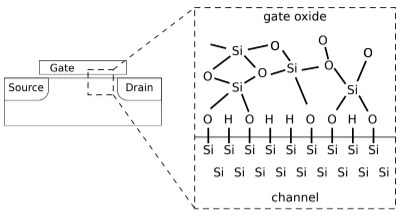
\includegraphics[scale=1]{figures/ReferencialTeorico/Cross section of a PMOS transistor.png}
    \caption{Seção da interface gate-substrato de um transistor PMOS. Fonte: \cite{Lorenz}}
    \label{fig:PmosCrossSec}
\end{figure}

Os estados de interface resultante deterioram parâmetros do transistor. Isso pode ser modelado pelo sistema RD, composto de dois processos: uma reação local e uma difusão dos produtos da reação.

A taxa de geração dessas interfaces é dada pela Equação \ref{eq:TaxaInteface}.

\begin{equation}
    \label{eq:TaxaInteface}
    \diff{N{\textsubscript it}}{t} = K{\scriptstyle F}(N{\scriptstyle 0} - N{\scriptstyle it}) - K{\scriptstyle R}N{\scriptstyle H}(0)N{\scriptstyle it}
\end{equation}

O primeiro termo do lado direito da equação mostra a componente de geração dos estados de interface, já o segundo termo descreve a regeneração das ligações, também denominada annealing reverso, uma característica especial do NBTI.

N\textsubscript{0} representa a quantidade inicial de ligações Si-H, N\textsubscript{it} representa o número de estados de interface e K\textsubscript{R} é a taxa constante de criação de ligações quebradas. No termo de recuperação N\textsubscript{H}(0) representa o número de átomos de hidrogênio na interface do silício com o óxido, K\textsubscript{R} é a taxa constante de annealing reverso das ligações incompletas e átomos de hidrogênio em ligações Si-H.

O lado direito da equação mostra que os estados de interface voltam a diminuir quando a condição de estresse é removida.

A criação de estados de interface é limitado pela difusão dos átomos de hidrogênio, como mostrado na Equação \ref{eq:TaxaDifusao}.

\begin{equation}
    \label{eq:TaxaDifusao}
    \diff{N{\textsubscript it}}{t} = - D{\scriptstyle H}\diff{N{\textsubscript H}}{x} + N{\textsubscript H}\mu{\textsubscript H}E{\scriptstyle ox}
\end{equation}

Onde D\textsubscript{H} representa o coeficiente de difusão, $\mu$\textsubscript{H} representa a mobilidade dos átomos de hidrogênio e E\textsubscript{ox} representa o campo elétrico que atravessa o óxido.

O segundo termo pode ser negligenciado para átomos ou moléculas eletricamente neutros. K\textsubscript{F}, K\textsubscript{R} e D\textsubscript{H} dependem da temperatura. K\textsubscript{F} também depende do campo elétrico aplicado. Isso demonstra que as interfaces só são geradas quando um campo elétrico é aplicado, o que não é necessário para o annealing e para a difusão.

As Equações \ref{eq:TaxaInteface} e \ref{eq:TaxaDifusao} formam um sistema que pode ser resolvido caso seja considerado que N\textsubscript{it} é muito menor que N\textsubscript{0}. A Equação \ref{eq:ResultanteRD} mostra a solução desse sistema e a dependência da quantidade de interfaces com relação o tempo.

\begin{equation}
    \label{eq:ResultanteRD}
    N{\textsubscript {it}} = \sqrt{\frac{K{\scriptstyle F}N{\scriptstyle 0}}{2K{\scriptstyle R}}}(D{\scriptstyle H}t)^{n}
\end{equation}

Onde n representa a constante exponencial de difusão e é sempre menor que 1, de forma que a geração das interfaces irá desacelerar com o tempo.

A variação Vth será proporcional ao N\textsubscript{it}, de forma que poderá ser escrito como mostrado na Equação

Porém, esse fenômeno não explica completamente a geração de NBTI. Um segundo mecanismo relacionado é baseado no aprisionamento de lacuna em defeitos no óxido pre-existentes ou provenientes de estresse elétrico \cite{Butzen}. O campo elétrico que gerado no gate quando o PMOS está negativamente polarizado causa o tunelamento de portadoras do canal nas falhas. Esse fenômeno vem sendo cada vez mais relevante na degradação por NBTI, considerendo que falhas no óxido são mais comuns em transistores high-k.

% Transistors with high-κ dielectric have higher density of pre-existing defects. From this point-of-view, hole trapping/detrapping is becoming the dominant contributor to NBTI degradation (KACZER, 2010).

Cada um desses fenômenos contribui para a variação da tensão de treashold resultando na equação \ref{eq:SomaVth}. Onde V\textsubscript{IT} á a contribuição das armadilhas de interface, V\textsubscript{HT} é a contribuição do aprisionamento em defeitos pré existentes e V\textsubscript{OT} é a contribuição do aprisionamento em defeitos gerados eletricamente.

\begin{equation}
    \label{eq:SomaVth}
    \Delta V{\textsubscript {th}} = \Delta V{\textsubscript {IT}} + \Delta V{\textsubscript {HT}} + \Delta V{\textsubscript {OT}}
\end{equation}

A Equação \ref{eq:VthTempo} mostra uma aproximação da variação da tensão de treshold ao longo do tempo considerando um nó tecnológico específico e um certo conjunto de condições ambientais \cite{Butzen}.

\begin{equation}
    \label{eq:VthTempo}
    \Delta Vth = A(TSP.t)^n
\end{equation}

Onde A é uma constante que depende da tecnologia, t é o tempo, n é a constante exponencia do NBTI e TSP é a probabilidade do transistor estar negativamente polarizado.
\subsubsection{Gerando NBTI}
\label{sec:GerandoNbti}
Muitos estudos já foram realizados para determinar em que condições o NBTI ocorre com mais facilidade em circuitos CMOS.

O fenômeno NBTI normalmente ocorre em transistores do tipo p operando com tensão de gate negativa em temperaturas variando de 100ºC a 250ºC \cite{Davidovic}. Os campos elétricos devem ser na faixa dos 6MV/cm, valores encontrados durante o burn-in do componente, porém com transistores cada vez menores, esses campos podem ocorrer durante a operação normal de dispositivos de alta performance \cite{Schroder}. A Figura \ref{fig:CampoEletricoAno} mostra o aumento do campo elétrico que atravessa o óxido em transistores CMOS ao longo dos anos.

\begin{figure}[H]
    \centering
    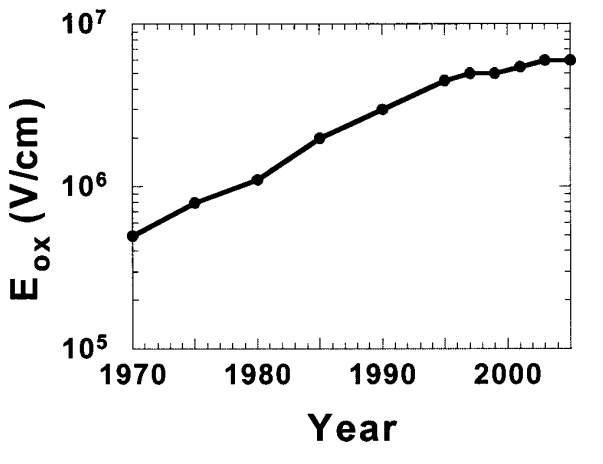
\includegraphics[scale=0.5]{figures/ReferencialTeorico/CampoEletricoAno.png}
    \caption{Campo elétrico no óxido em dispositivos CMOS ao longo dos anos. Fonte: \cite{Schroder}}
    \label{fig:CampoEletricoAno}
\end{figure}

% Typical stress temperatures lie in the 100– 250 °C range with oxide electric fields typically below 6 MV/cm, i.e., fields below those that lead to hot carrier degradation. Such fields and temperatures are typically encountered during burn in, but are also approached in highperformance ICs during routine operation.

Para aplicar o efeito de NBTI no dispositivo ensaiado no trabalho \cite{Davidovic}, os pesquisadores o estressaram por 2000 horas, aplicando tensões negativas de 30 a 45V no gate (com fonte e dreno aterrados) em uma temperatura de variando de 125 a 175ºC.

O trabalho de \cite{Bhardwaj} desenvolveu um modelo preditivo para NBTI em dispositivos CMOS de nó tecnológico de 45nm, que alcançou estimativas precisas da degradação em longo prazo da tensão de threshold de transistores PMOS devido ao fenômeno.

Um outro trabalho \cite{Grossi}, realizou simulações para analisar os efeitos do BTI em amplificadores operacionais, e viu que o ganho DC, a frequência de corte e o slew rate são significativamente degradados em AMPOPs operando em malha aberta. Já para Ampops operando com realimentação negativa apenas a frequência de corte mostrou uma degradação significativa.

Alguns trabalhos, inclusive, realizaram estudos dos efeitos de NBTI em osciladores em anel. Um deles \cite{Lorenz} mostra uma degradação de 5\% com 144 horas de exposição à 125°C. Já outro \cite{Sato}, que estudou métodos para diminuir o efeito de NBTI em osciladores em anel, resultou uma degradação de 0,25\%, com 42 horas de exposição, porém à apenas 85°C. Um terceiro trabalho \cite{Linder} propõe topologias de osciladores em anel que permitem estudar em separado os efeitos do PBTI, nele foi medida um degradação de 1,8\% considerando apenas o PBTI, 2,2\% considerando apenas o NBTI e 3,9\%  considerando apenas os dois efeitos combinados tendo sido realizado um estresse de 2 horas e 47 minutos (10000 segundos) segundos à 125°C.


\chapter{Metodologia}
Neste capítulo serão descritos os procedimentos utilizados para verificar os efeitos de envelhecimento acelerado nos FPGAs de interesse.

\section{Desenvolvimento dos Osciladores em Anel}

A topologia de oscilador em anel foi escolhida para os testes por sua disseminada utilização na caracterização de dispositivos MOSFET. Seu uso é amplo, pois medidas a utilizando se aproximam muito mais de aplicações reais do que medições paramétricas DC padrões.

Foram realizados testes preliminares com diferentes quantidades de inversores para encontrar uma quantidade apropriada, pois, com poucos osciladores não há tempo suficiente para os inversores chavearem e com muitos osciladores o limite de iterações que as IDEs permitem era atingido.

Considerando isso, foi decidido que em cada um dos dispositivos foi sintetizado dois osciladores, um com 1001 inversores e outro com 4999. A escolha de utilizar dois osciladores em cada FPGA foi tomada por dois motivos: para se ter certeza que as IDEs não estavam simplificando os estágios inversores do circuito sintetizado e para verificar que o envelhecimento afeta igualmente diferentes partes do FPGA.

A grande quantidade de inversores é relevante, pois assim as pequenas variações aleatórias nas características de cada transistor que compõe os dispositivos tenderão a se diluir.

\subsection{Desenvolvimento do Código para os Osciladores}

Para desenvolver e sintetizar os osciladores em anel foi utilizada a linguagem de descrição Verilog. Para o Cyclone II foi utilizada a IDE Quartus II versão 12.1, já para o ZedBoard foi utilizada a IDE Vivado versão 2023.1.

O Quadro \ref{code:RingOsc} mostra o código desenvolvido em Verilog para o módulo que implementa o oscilador em anel com N inversores. O mesmo código foi utilizado para os dois FPGAs nas duas IDEs diferentes.

\begin{lstlisting}[label={code:RingOsc}, style=VerilogStyle, caption={Módulo do Oscilador em Anel. Fonte: O Autor}]
module RingOscillator 
	#(parameter N = 5)
	(
		input  en,
		output reg and_1    /*synthesis keep*/
	);
	reg [N - 1:0] notGate /*synthesis keep*/;
	integer i;
	generate
	  always @ (*) begin
		  and_1 <= en & notGate[N - 1];
	  	notGate[0] <= ~and_1;
	  	for (i = 1; i < N; i = i + 1)   begin: inverter_chain
			  notGate[i] <= ~notGate[i - 1];
		  end
	  end
	endgenerate
endmodule
\end{lstlisting}

O módulo possui uma entrada en, responsável por habilitar o circuito, uma saída and\_1 que é a saída da porta and do circuito, de onde o sinal do oscilador é obtido. O valor N é parametrizável, o que permite a reutilização do mesmo código para osciladores com diferentes números de inversores.

São então instanciadas N registradores, que serão utilizados para criar os inversores. O registrador and\_1 recebe o resultado da operação E lógica do sinal de enable e a saída do último inversor. O primeiro inversor é definido como o registrador and\_1 invertido.

Um bloco 'for' é utilizado para automatizar as atribuições dos inversores seguintes, sendo a cada um atribuído o valor inversor anterior negado.

Um ponto importante de destacar é a necessidade de utilizar diretivas de compilação para impedir que os inversores sejam simplificados na síntese. Essas diretivas são diferentes em cada uma das IDEs, na Quartus II é utilizado a diretiva /* synthesis keep */ e na Vivado é utilizado a diretiva /* synthesis syn\_keep=1 */.

Na Figura \ref{fig:DE2Imp3Osc} pode ser visto como o Quartus II implementa em hardware o código do Quadro \ref{code:RingOsc} para um N igual a 3. A implementação é feita através de portas lógicas comuns, o que é diferente da implementação feita pelo Vivado, como visto na Figura \ref{fig:ZedImp3Osc}, que utiliza LUTs de uma variável para representar os inversores.

\begin{figure}[H]
    \centering
    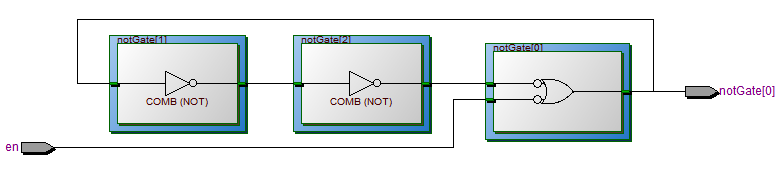
\includegraphics[width=\linewidth]{figures/Metodologia/DE2_Implementation_3Inverter_Gates.png}
    \caption{Síntese do módulo de alto nível gerado no Quatus II. Fonte: O Autor}
    \label{fig:DE2Imp3Osc}
\end{figure}

\begin{figure}[H]
    \centering
    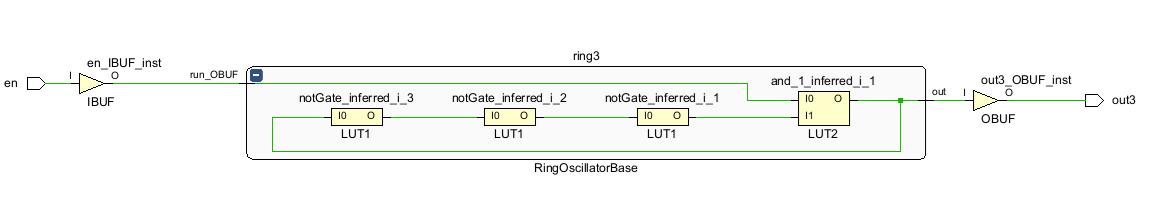
\includegraphics[width=\linewidth]{figures/Metodologia/ZedBoard_Implementation_3Inverter.png}
    \caption{Síntese do módulo de alto nível gerado no Vivado. Fonte: O Autor}
    \label{fig:ZedImp3Osc}
\end{figure}

O Quadro \ref{code:TopLevel} mostra o módulo de alto nível em que é instanciado dois osciladores em anel, um com 1001 e outro de 4999 inversores. 

\begin{lstlisting}[label={code:TopLevel}, style=VerilogStyle, caption={Estanciamento dos Módulos. Fonte: O Autor}]
module TopLevel
	(
		input en,
		output run,
		output out1001, out4999
	);
	
	assign run = en;

	RingOscillator #(.N(1001)) ring1001(en, out1001);
	RingOscillator #(.N(4999)) ring4999(en, out4999);
endmodule
\end{lstlisting}

O módulo possui uma entrada 'en', responsável por habilitar o circuito, uma saída 'run', usada para indicar que o circuito está em funcionamento e as saídas dos dois osciladores 'out1001', 'out4999'. Também são declaradas duas instâncias do módulo desenvolvido no Quadro \ref{code:RingOsc}.

As Figuras \ref{fig:DE2RtlSchem} e \ref{fig:ZedRtlSchem1} mostram, respectivamente, o circuito implementado pelo software Quartus II e Vivado para o módulo de alto nível que serão utilizado nos FPGAs.

\begin{figure}[H]
    \centering
    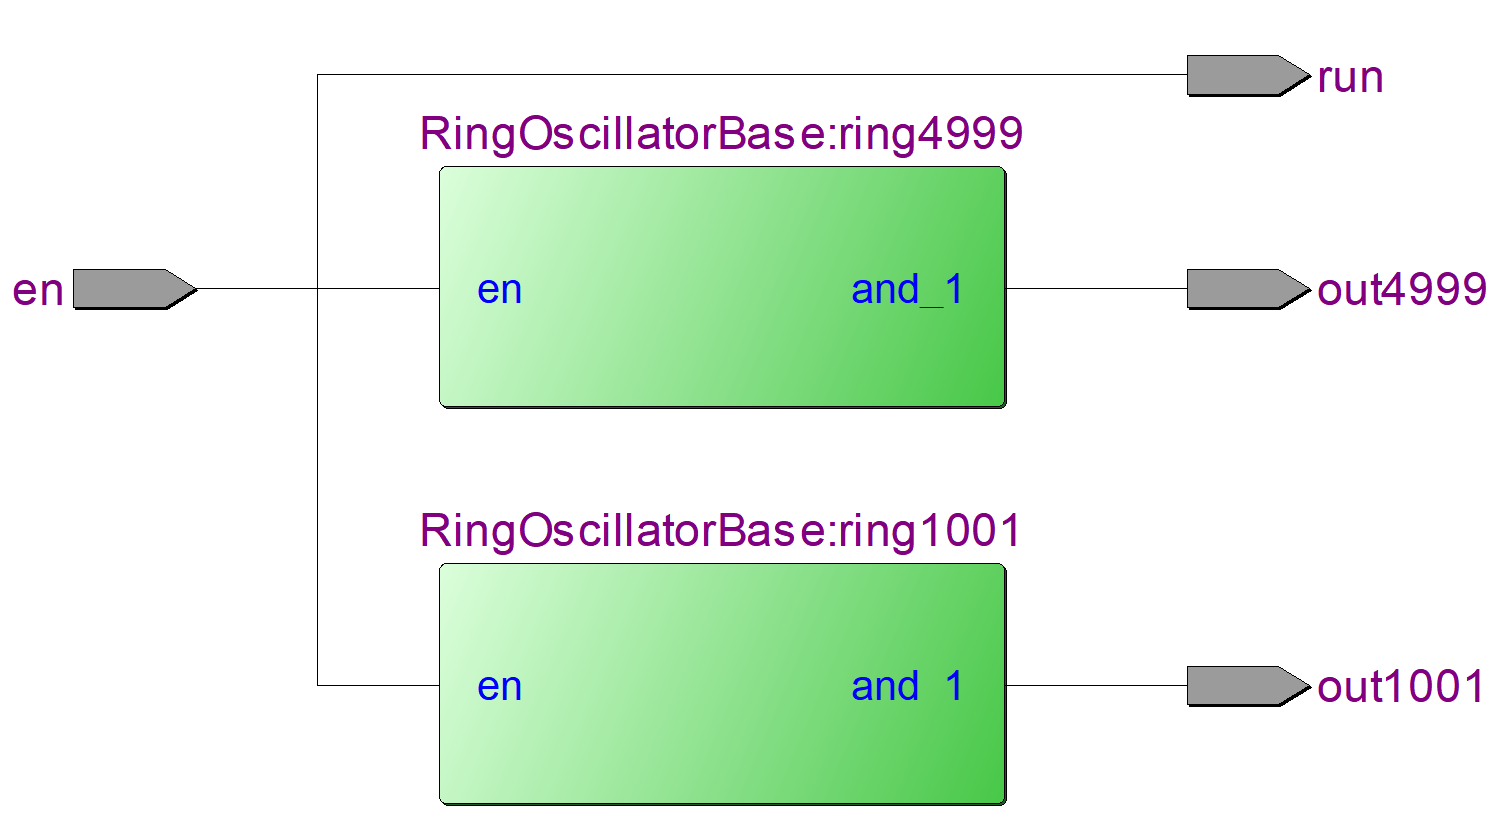
\includegraphics[scale=0.25]{figures/Metodologia/DE2_RTL_Schematic.png}
    \caption{Síntese de um oscilador com três inversores gerado no Quatus II. Fonte: O Autor}
    \label{fig:DE2RtlSchem}
\end{figure}

\begin{figure}[H]
    \centering
    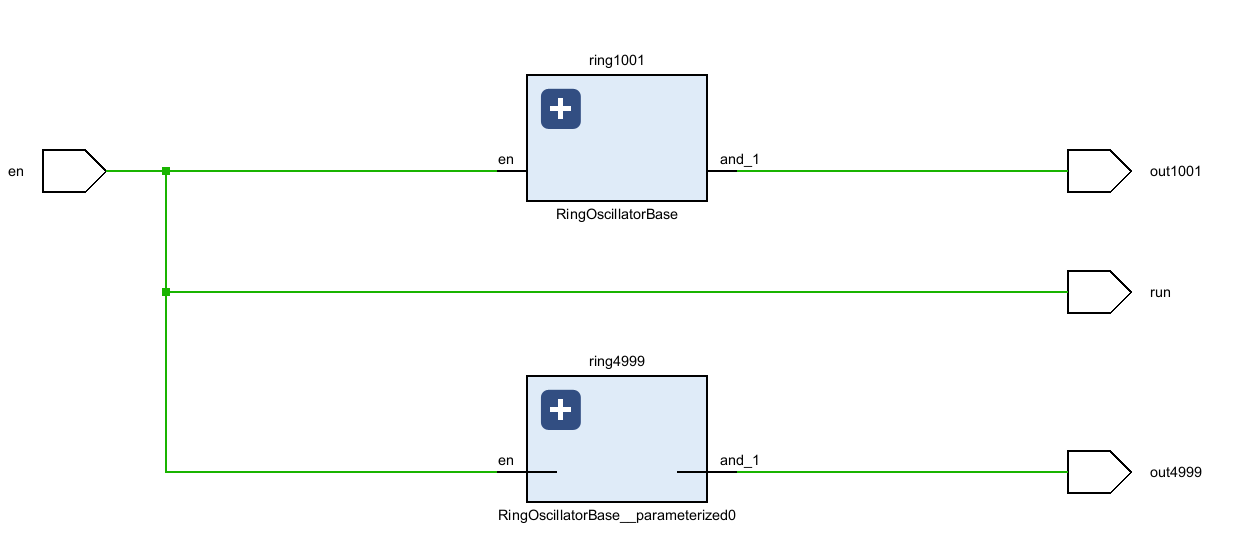
\includegraphics[width=\linewidth]{figures/Metodologia/ZedBoard_RTL_Schematic.png}
    \caption{Síntese de um oscilador com três inversores gerado no Vivado. Fonte: O Autor}
    \label{fig:ZedRtlSchem1}
\end{figure}

Nas duas placas a entrada 'en' foi atribuída a um pino do FPGA ligado a uma chave, a saída 'run' foi atribuída a um pino do FPGA ligado a um LED e as saídas 'out1001' e out4999 foram atribuídas a pinos do FPGA ligados a conectores de entrada e saída de uso geral.

Após o desenvolvimento, o circuito sintetizado foi simulado utilizando a ferramenta apropriada para cada um dos componentes. Constatada a validade da solução ela foi transferida para os FPGAs reais e será medida, através de um osciloscópio, a frequência de oscilação das saídas do circuitos.
\section{Ensaios de Envelhecimento}

Para induzir o fenômeno de BTI nos dispositivos foi utilizada uma câmara térmica para ensaios com componenentes eletrônicos. Inicialmente a temperatura de exposição foi de 100°C, temperatura que é inferior a faixa de ocorrência do BTI, mas que foi utilizada para verificar se os componentes não iriam ser danificados com a temperatura.

A Figura \ref{fig:CamTerm} mostra a câmera térmica utilizada para os ensaios. Ele foi fabricado pela SPX Thermal Product Solutions e alcança temperaturas de -75ºC a 200ºC

\begin{figure}[H]
    \centering
    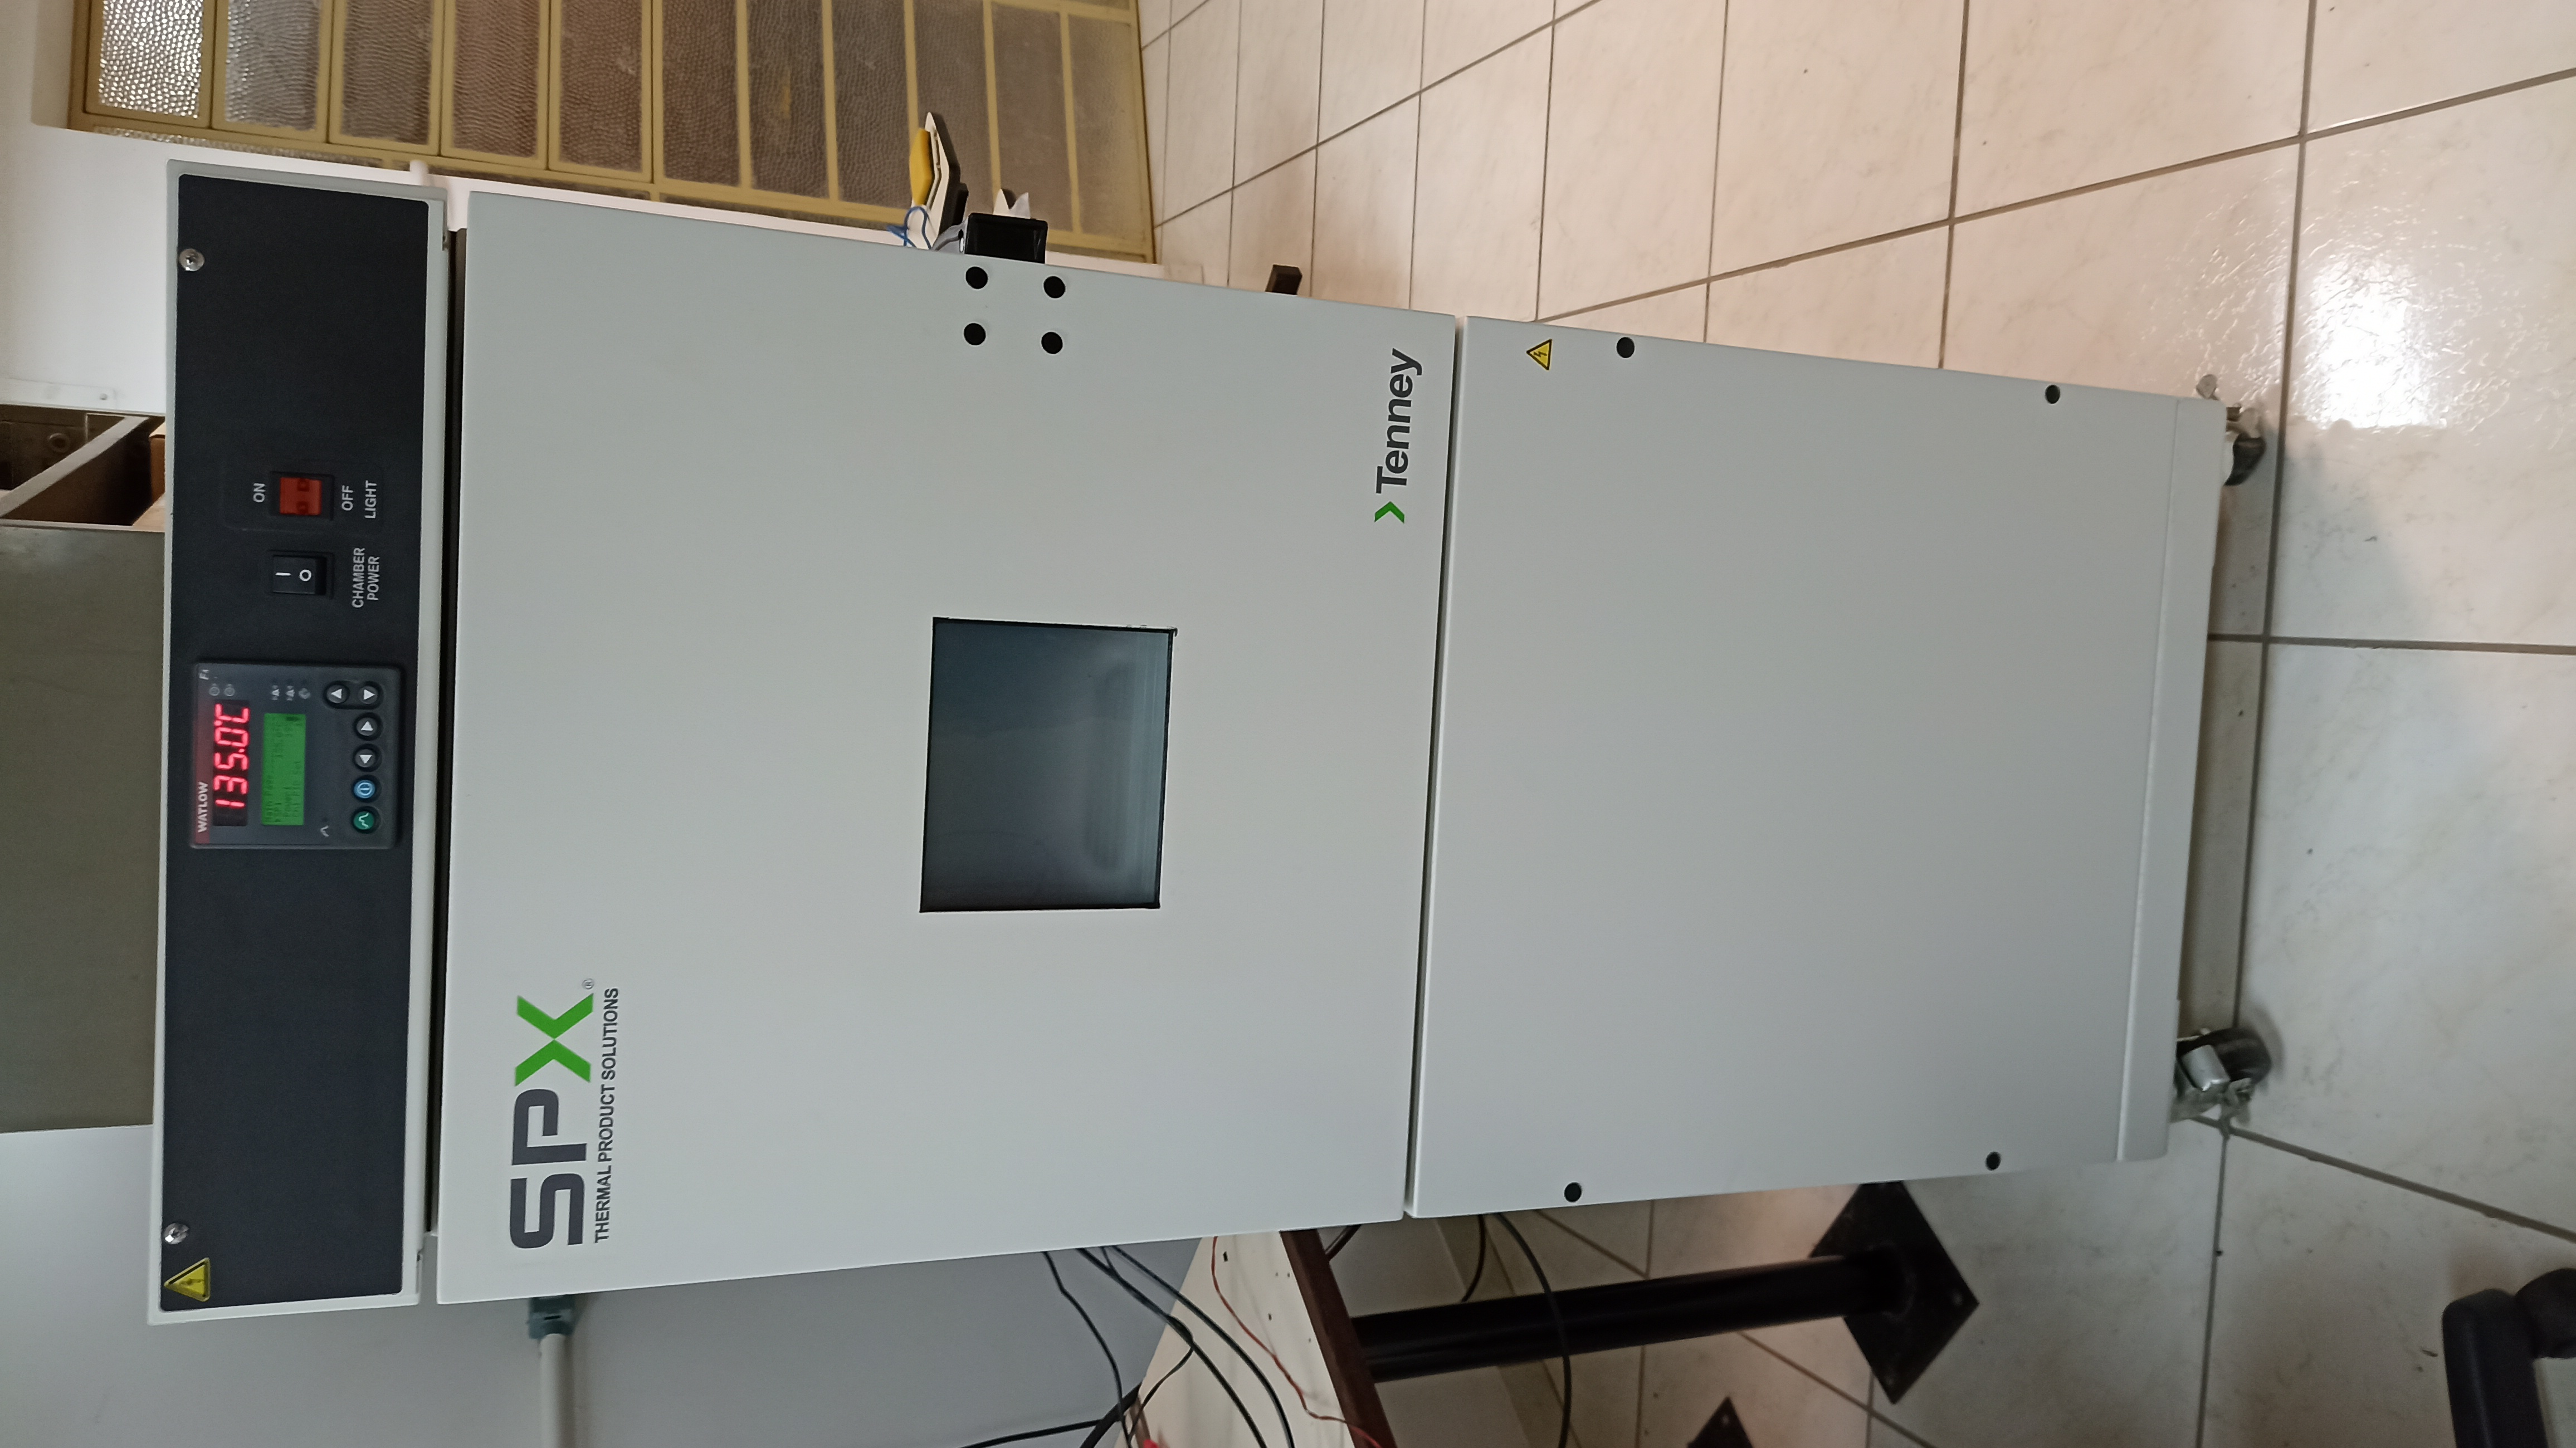
\includegraphics[angle=270, scale=0.08]{figures/Ensaios_CamaraTermica.jpg}
    \caption{Câmara térmica utilizada para os ensaios. Fonte: O Autor}
    \label{fig:CamTerm}
\end{figure}

Constatando que não houve problema à 100ºC, a temperatura foi aumentada para 125°C. Como também não houve danos, a temperatura foi, então, elevada para 135°C.

Nessa temperatura foi observado que o conector de alimentação da placa DE2 apresentava sinais de derretimento, por isso, a temperatura dos ensaios foi definida em 135°C. Temperatura que está dentro da faixa de 125 e 175ºC que a bibliografia indica como sendo a faixa em que o BTI ocorre mais facilmente.

O tempo que os dispositivos forem expostas ao calor não foi contínua, devido a impossibilidade de ficar durante a noite no laboratório e, por motivos de segurança, de deixar a câmara térmica ligada sem supervisão. Portanto os dispositivos, de forma geral, foram expostos à câmara térmica durante o dia e retirados dela durante a noite, ficando ligados o tempo todo, de forma que não houvesse relaxamento.

Outras duas placas, dos mesmo modelos das ensaiadas, foram deixadas fora da câmara térmica pelo mesmo tempo, sempre ligadas e com os mesmos osciladores em anel sintetizados. Comparar as medidas entre as placas que foram aquecidas com as que nao foram é importante para verificar que se a degradação na frequência é proveniente do estresse térmico ou se é apenas resultado do funcionamento prolongado.

A câmara térmica permite realizar medidas nos dispositivos ensaiados enquanto eles estão dentro dela. Portanto foi possível medir a frequência dos osciladores em anel durante o processo de estresse térmico.

Enquanto a câmara aquece da temperatura ambiente pra temperatura alvo, as medições foram mais frequentes, de cinco em cinco minutos. Quando a temperatura alvo é atingida as medidas ficam mais esparsas.

É importante separar os efeitos instantâneos da temperatura na frequência dos osciladores do efeito a longo prazo do BTI. Por isso é necessário comparar as medidas feitas em uma mesma temperatura. O momento que a temperatura é a mais estável é quando a câmara já chegou aos 135°C.

Outra comparação relevante é a das curvas frequência por temperatura ao longo de cada ciclo.

Comparando essas medidas em relação ao tempo total estressado será possível constatar se houve ou não uma degradação na frequência de funcionamento dos dispositivos. E se houve uma diferença significativa na degradação entre as duas placas.

Após os ensaios de envelhecimento foi realizado um ensaio para medir a recuperação dos circuitos, para verificar quanto da degradação sofrida é reversível. Para isso as quatro placas foram desligadas e deixadas em temperatura ambiente. Medidas ao longo do tempo foram realizadas até o tempo de relaxamento totalizar o tempo total que as placas foram estressadas.

\begin{figure}[H]
    \centering
    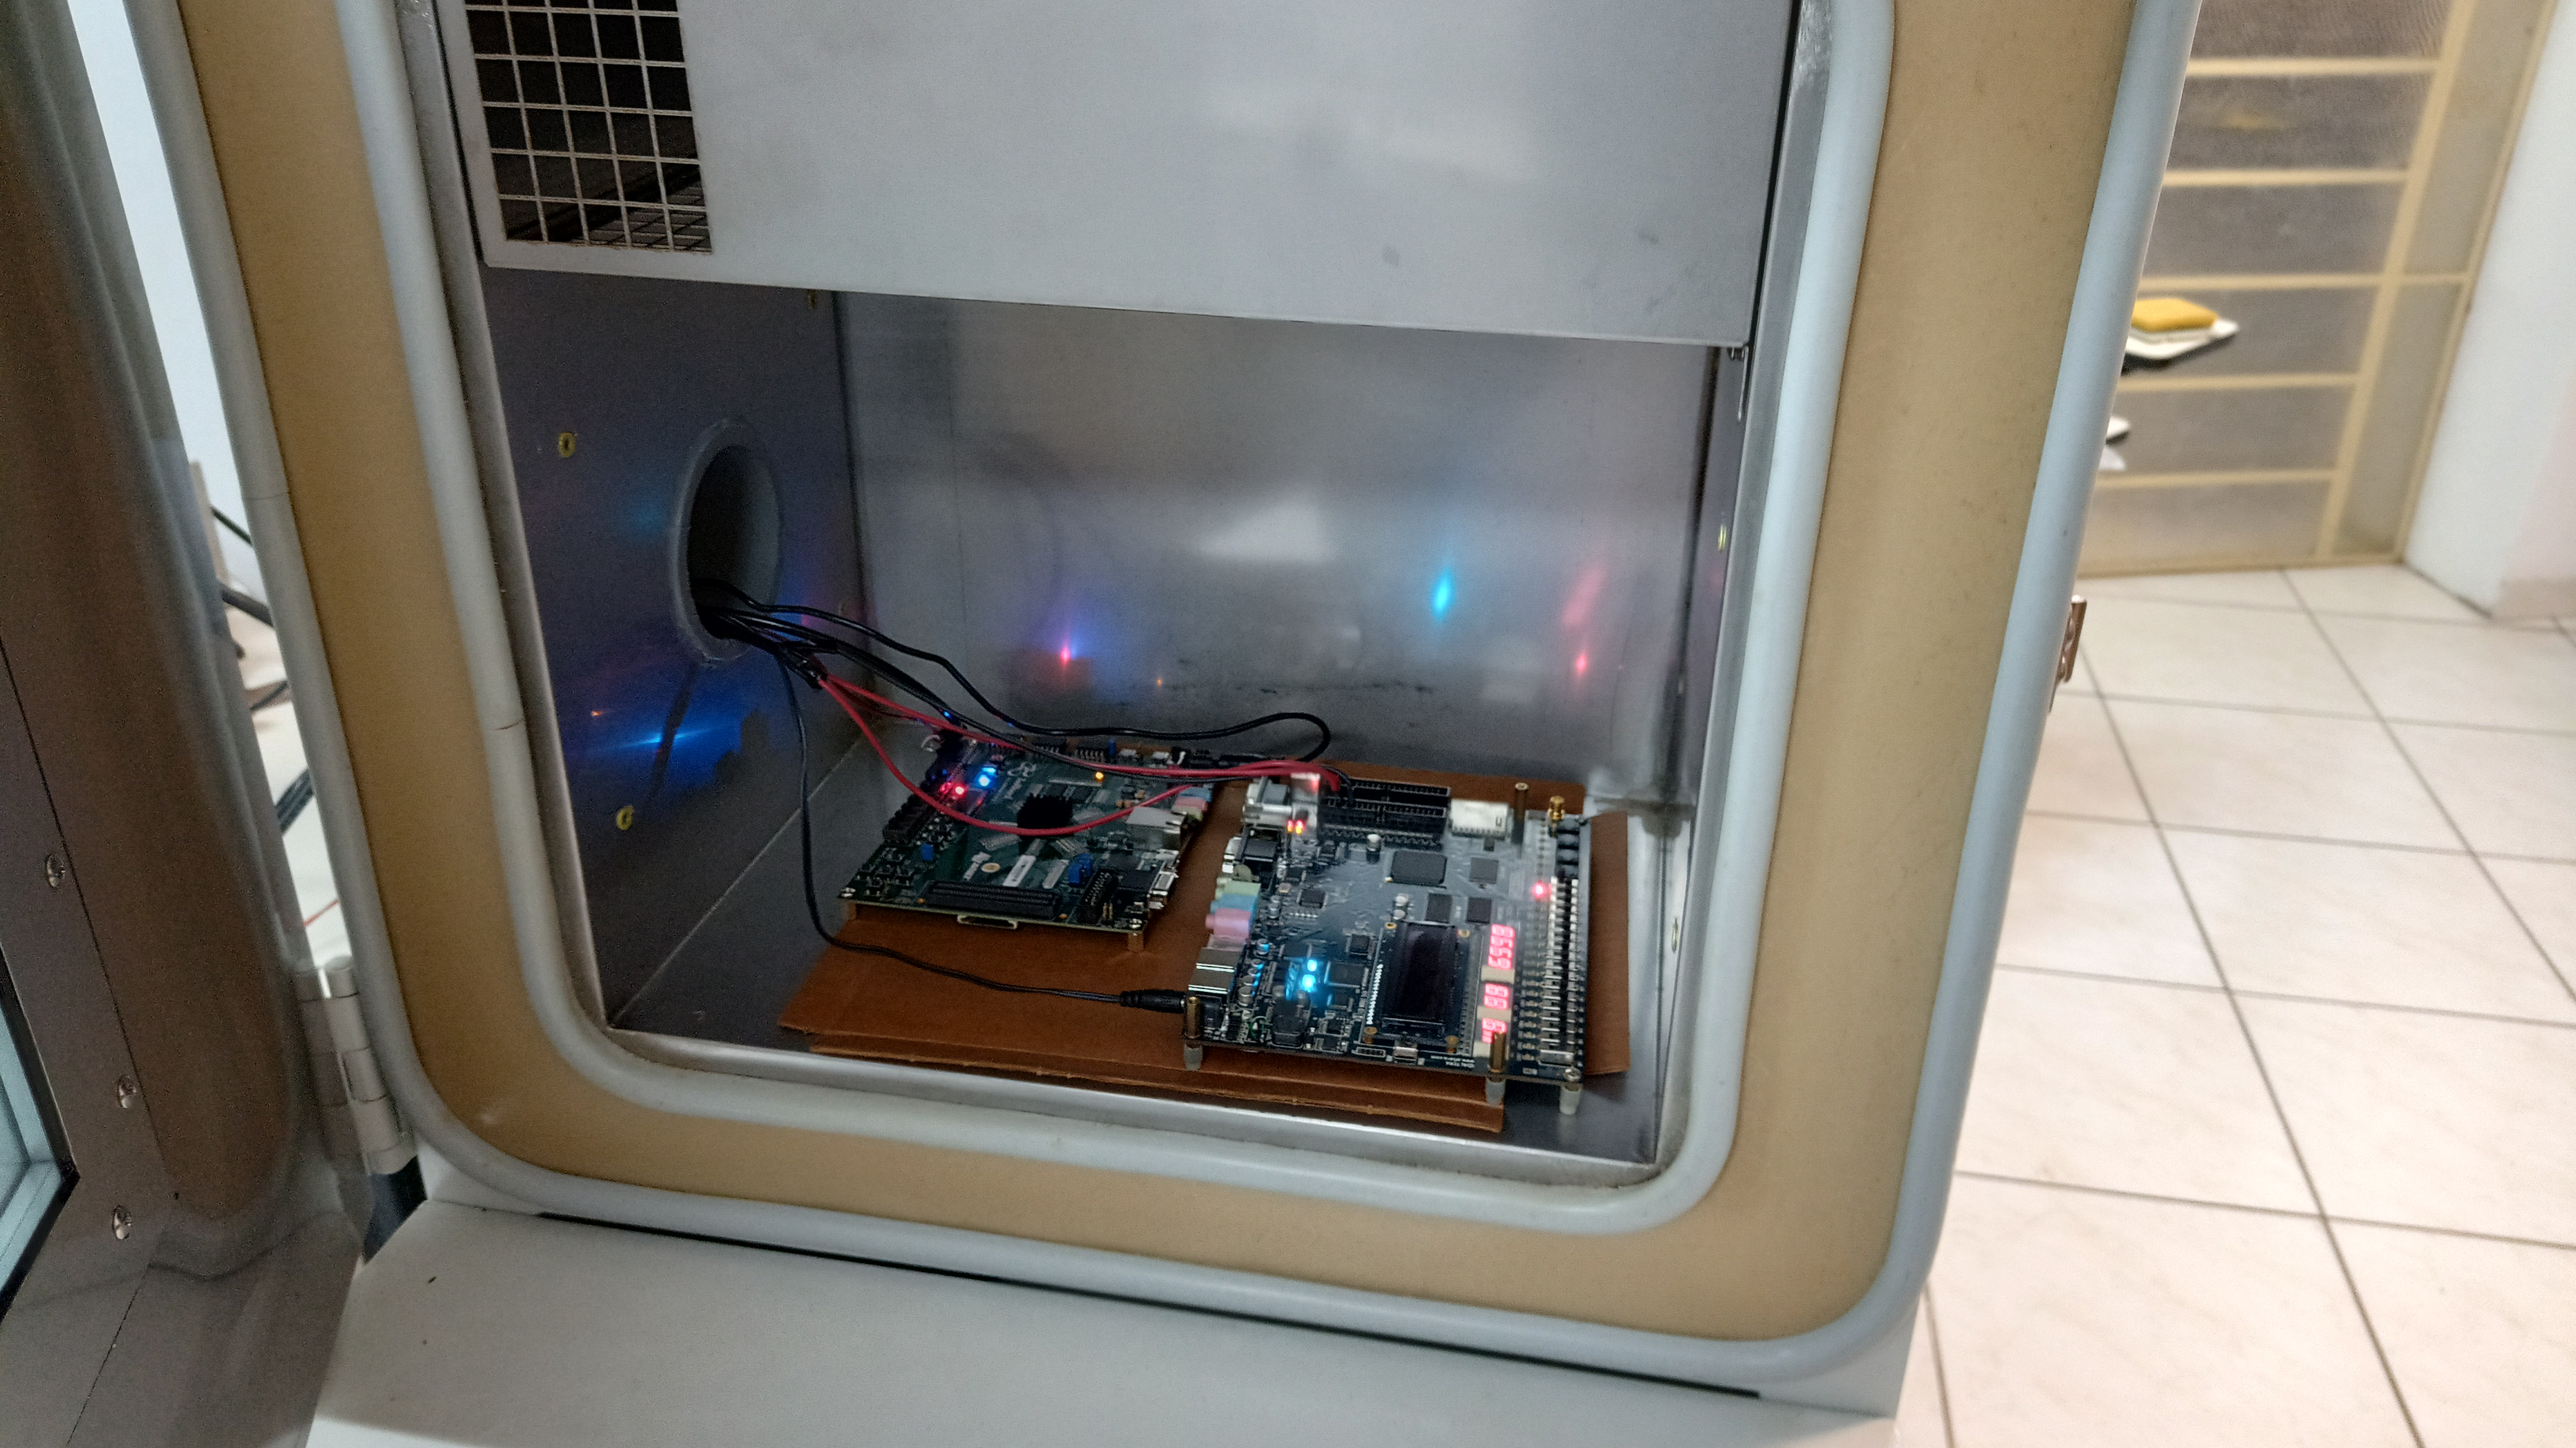
\includegraphics[width=\linewidth]{figures/Ensaios_FpgasNoForno.jpg}
    \caption{FPGAs dentro da Câmara térmica. Fonte: O Autor}
    \label{fig:CamTerm}
\end{figure}

\begin{figure}[H]
    \centering
    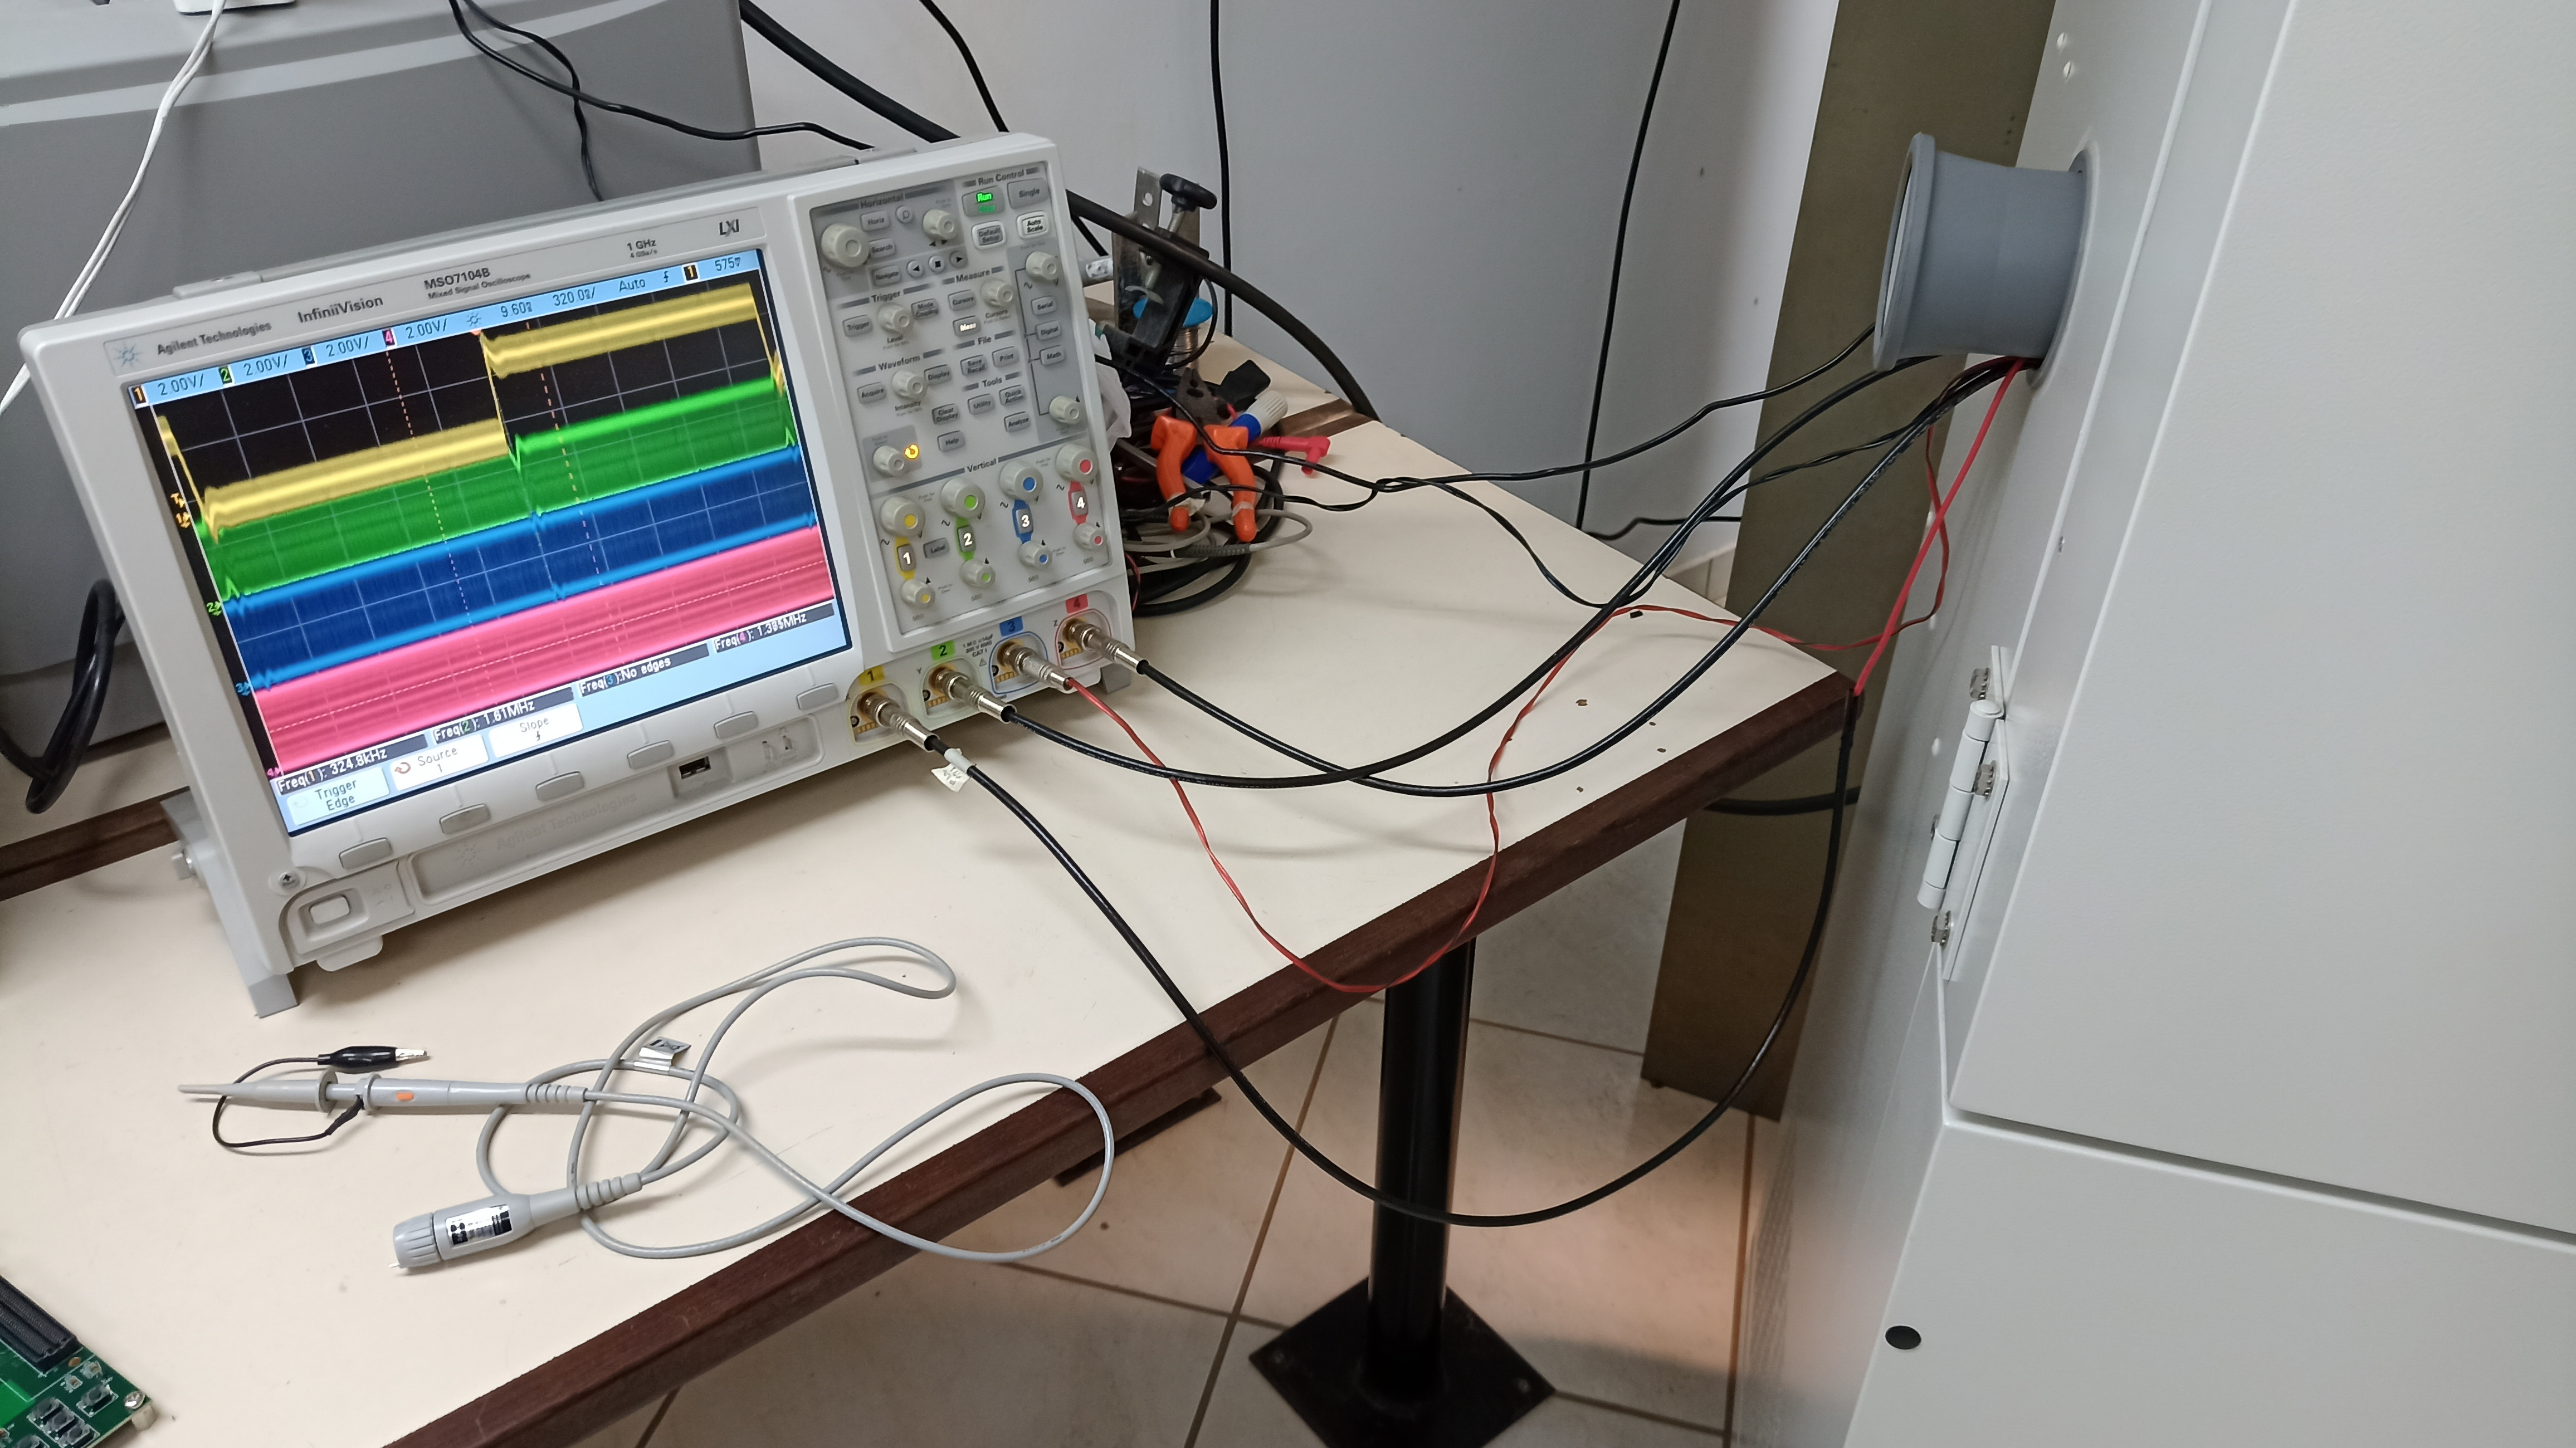
\includegraphics[width=\linewidth]{figures/Ensaios_Osciloscopio.jpg}
    \caption{Osciloscópio utilizado para as medidas. Fonte: O Autor}
    \label{fig:CamTerm}
\end{figure}


% \chapter{Resultados}

%\bibliographystyle{bib/ref}
\bibliography{bib/ref.bib}
\begin{listofabbrv}{M2(CN2)M}
        \item[FPGA] Field-Programmable Gate Array
        \item[MOSFET] Metal Oxide Semiconductor Field Effect Transistor
        \item[CMOS] Complementary Metal Oxide Semiconductor
        \item[PMOS] Positive Metal Oxide Semiconductor
        \item[NMOS] Negative Metal Oxide Semiconductor
        \item[BTI] Bias Temperature Instability
        \item[PBTI] Positive Bias Temperature Instability
        \item[NBTI] Negative Bias Temperature Instability
        \item[RD] Reaction Diffusion
        \item[IDE] Integrated Development Environment
        \item[TDDB] Time-Dependent Dielectric Breakdown
        \item[EM] Electromigration
        \item[HCI] Hot Carrier Injection
\end{listofabbrv}
%\input{chapters/07_appendix.tex

\end{document}
